%!TEX root = ../../../thesis.tex

The work throughout the remainder of this thesis is based upon an interface model put forward by my supervisor and a colleague of his, Peter Single.
The model was verified in a single, known concentration of phosphate buffered saline at the point I began using it.
Working through the processes taken by my supervisor to create his model, I re-created the model from the ground up.
By creating a range of solutions of buffered saline to test against, I fitted parameters of the initial model to the concentration of saline.
This put me in a good position to compare saline solutions to live biological solutions.
That comparison is the main scientific contribution resulting from this work.

\section{The Scott-Single Interface Model}

  \begin{figure}
    \centering
    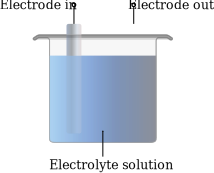
\includegraphics{content/pt2/07-InterfaceModel/graphics/electrode-electrolyte}
    \caption{\label{fig:electrode-electrolyte}Electrodes submerged in an electrolyte solution, such a system can be described by the Scott-Single Interface Model.}
  \end{figure}

  Jonathan Scott and Peter Single recently published an electrical model of an implantable electrode array in saline in 2013 \cite{ScottSingle2013}.
  The intention of that model was to simulate the electrical impedance that a medical implant device would see once implanted into a human spinal cavity.
  It is also general enough to use in any situation where electrodes are placed in an electrolyte solution, such as depicted in \cref{fig:electrode-electrolyte}.

  \begin{figure}
    \centering
    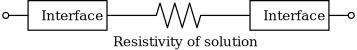
\includegraphics{content/pt2/07-InterfaceModel/graphics/simpleElectrodeElectrolyteModel}
    \caption{\label{fig:pt2-simpleElectrodeElectrolyteModel}Connection diagram of two electrodes (with their interface models) connected together by the resistivity of an electrolyte solution.}
  \end{figure}
  The model comes in two parts, the electrode interface, and the resistivity of the electrolyte's bulk.
  \Cref{fig:pt2-simpleElectrodeElectrolyteModel} shows the general electrical configuration of such an electrode-electrolyte system.
  It shows that there are two interfaces per system, and that the liquid side of those two interfaces are joined electrically by the resistance of the electrolyte's bulk resistivity.
  The metal side of the interfaces is what the rest of the circuit would connect to.
  First, the interface model will be explained.


  \subsection{The interface model}

    \begin{figure}
      \centering
      \includegraphics{content/pt2/07-InterfaceModel/graphics/interfaceSchematic}
      \caption{\label{fig:pt2-interfaceSchematic}Electrical schematic of the electrode-electrolyte interface}
    \end{figure}

    The full interface model is represented schematically by \cref{fig:pt2-interfaceSchematic}.
    It represents the transition between the metal of the electrode and the liquid of the electrolyte.
    The model used throughout this thesis is a slightly simplified version of \cref{fig:pt2-interfaceSchematic} in that the memristors have been removed.





    % The Scott-Single interface is modelled by the circuit shown in \cref{fig:pt2-interfaceSchematic}.
    % Each of the components and their functions will be explained in the coming sections.
    % It is important to realise that this model only represents a single interface between metal and electrolyte.
    % By itself it is incapable of simulating any useful electrode/electrolyte system.
    % For that, a minimum of two interfaces must be used - one as a cathode and one as an anode.
    % Additionally, some model of the electrolyte resistivity needs to connect the two interfaces.


    % \Cref{fig:pt2-simpleElectrodeElectrolyteModel} shows the smallest/simplest use of the interface model.
    % This configuration represents two electrodes placed in an electrolyte solution.
    % It allows simulation of impedance between those electrodes and can be connected to other electronic circuits.
    % A model like this is only valid for a two electrode system.
    % Because the electrode array in our application has eight electrodes, the model is more complex.
    % In full, that model will have eight electrode interfaces and a resistor network connecting each interface.

    \subsubsection{Interface series resistance: Resistor}
      The series resistor at the right hand side of the model schematic (labelled $R_{S}$) represents the purely resistive component of the interface's impedance.
      As it is series with all other components in the interface model, there is no way for charge to cross the interface without encountering this resistance.

    \subsubsection{Polar effects: Constant phase element}
      At the centre of the model is the constant phase element, or CPE.
      This element behaves like a capacitor, except its impedance magnitude does not decay at \SI{20}{\decibel} per frequency decade like a conventional capacitor does.
      They are primarily used to describe the capacitance of double layer interfaces, the function it serves in this model.
      These elements may also prove useful in describing the nature of battery and super-capacitor behaviour.
      A CPE is not an element found in the field electronic engineering and therefore must built from existing components.
      \begin{figure}[h]
        \centering
        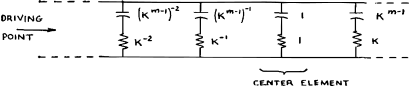
\includegraphics{content/pt2/07-InterfaceModel/graphics/Morrison-RC}
        \caption{\label{graph:pt2-morrisonCPE}Ralph Morrison's implementation of a constant phase element using an infinite array of resistor-capacitor pairs (taken from Morrison's paper -- \cite{Morrison1959}).}
      \end{figure}
      In 1959, Morrison demonstrated a way of creating constant phase elements from an infinite array of resistor-capacitor (RC) pairs \cite{Morrison1959}.
      One of Morrison's implementations of a constant phase element is presented as \cref{graph:pt2-morrisonCPE}.
      Each parallel branch has precisely chosen resistor and capacitor values such that when summed together the impedance magnitude versus frequency is a constant slope, i.e., the impedance does not flatten at a particular frequency as it would with a single RC pair.
      Creating any element comprised of an infinite number of sub-elements is not possible, but by selecting only those elements that contribute to the bandwidth of interest the result is the same within the selected frequency window.
      Using that method and selecting only RC pairs with a cut-off frequency in the range of \SI{1}{\milli\hertz} to \SI{1}{\mega\hertz}, a practical CPE element is created.

      \begin{figure}
        \centering
        \includegraphics{content/pt2/07-InterfaceModel/graphics/graph_cpe_creation}
        \caption{\label{graph:pt2-cpe_creation}Graph showing how a non \SI{20}{\decibel} per frequency decade}
      \end{figure}

      \Cref{graph:pt2-cpe_creation} shows the individual contributions from each RC branch in an implementation of a CPE.
      Each of grey trace represents a single RC branch in the CPE element, each displaying a high-pass filter slope.
      The value of the resistor in each branch is evident by the vertical spacing of the traces, clearly visible to the right of the graph.
      The branches in this particular example have been spaced in the frequency domain at a density of three per decade, as shown by the black crosses.
      This means that per decade of frequency, there are three corner frequencies, each relating to an RC pair.
      Because each of there branches are in parallel the total response of the CPE is the sum of each branch, that response is shown as the black trace on the graph.
      The critical observation is that the slope of the resulting trace is not the same as each of the individual branches.
      This allows the CPE to behave fractionally as a capacitor, being anywhere between resistive (flat response) and capacitive (\SI{20}{\decibel}/decade slope).

      The CPE is represents readily reversible reactions, polar reorientation, and ionic repulsion and attraction between the electrode surface and electrolyte.
      It is capacitive in nature because each of these mechanisms store charge, which can be drawn back by reversing the applied electromotive force.


    \subsubsection{Faradaic reactions: diodes}
      If the voltage placed across the interface is kept within certain limits, the CPE and series resistance ($R_{S}$) would be all that is necessary to accurately mimic a single electrode-electrolyte interface.
      But once the electric potential across the interface becomes high enough, Faradaic reactions will occur at the electrode's surface.
      Faradaic reactions are reactions involving charge transfer, adding ionised species to the electrolyte and often producing gas.
      Gas, or any new species, is to be avoided in an implanted setting as this causes damage to the patient.
      The rate at which a specific reaction occurs increases exponentially with electrode overpotential.
      Because that reaction is a means of transporting electrical current between the electrodes, the current draw also increases exponentially.

      \begin{equation}
        I = I_{S}\left( e^{V_{D}/n V_{T}} - 1\right)
        \label{eqn:pt2-diodeEquation}
      \end{equation}

      Exponential current draw with increasing voltage is the transfer characteristic of a diode.
      The standard diode equation is shown as \cref{eqn:pt2-diodeEquation} where $I$ is the current through the diode,
      $I_{S}$ is the reverse saturation current,
      $V_{D}$ is the voltage across the diode,
      $n$ is the diode's ideality factor,
      and $V_{T}$ is the thermal voltage.
      The model make use of this transfer function to mimic the current draw associated with Faradaic reactions.
      As a diode has the characteristic that it only conducts current in one direction, it represents one specific reaction happening in one direction.
      Because the electrode/electrolyte reactions are often reversible, a pair of diodes is used; one diode for each direction.

      As Faradaic reactions are to be avoided in the implanted setting, only their onset needs to be included in the model.
      Essentially this means that we only need to add diodes to the model that mimic the current/voltage curve associated with the first Faradaic reaction of the system.
      It is not important what that specific reaction is, only that we can enter its characteristics into the model.
      Detecting the onset of that exponential current via measurement is necessary in order to identify the diode parameters.
      If it where necessary to model other Faradaic reactions then additional pairs of diodes can be added to the model, each in parallel with the existing pair.
      The additional diodes would have a unique set of parameters governing their behavior.

    \subsubsection{Species depletion: memristors}
      Because Faradaic reactions are by definition \emph{reactions}, they must consume reactants to produce the reaction products.
      Depending on the volume of electrolyte available


  \subsection{Inter-electrode resistivity}
    \begin{figure}
      \centering
      \includegraphics{content/pt2/07-InterfaceModel/graphics/StJudeOctrodeDiagram}
      \caption{\label{fig:StJudeOctrode_Labelled}St. Jude Medical Octrode. An eight electrode array commonly used in spinal stimulation implants.}
    \end{figure}

  % \Cref{fig:StJudeOctrode_Labelled} is an illustration of the electrode array and the numbering scheme used to identify each electrode.
  % Each electrode on this array is made from platinum and is separated by an insulating spacer.
  % The array has eight platinum wires that run through the cable to each of the electrodes.
  % This electrode was used through the remainder of this thesis and is the electrode used by Saluda in medical trials of their stimulators.

  % \begin{figure}
  %   \centering
  %   \includegraphics{content/pt2/07-InterfaceModel/graphics/interfaceSchematic_noMemristive}
  %   \caption{\label{fig:pt2-interfaceSchematic_noMemristive}Electrical schematic of the electrode-electrolyte interface with the memristors omitted}
  % \end{figure}

  % Figure \cref{fig:pt2-interfaceSchematic_noMemristive} shows a simplified version of the interface model.
  % It is simplified in that it does not include the memristors of the original model.
  % A memristor is a relatively new type of electronic device which hasn't made it to consumer electronics yet.
  % It behaves like a resistor that alters it's resistance depending on the sum of current that it passes.

\section{Methods of Parameter Extraction}
  \subsection{Resistivity and constant phase element}
  \subsection{Faradaic currents}

